\documentclass[a4paper]{article}

\usepackage[english]{babel}
\usepackage[UKenglish]{isodate}
\usepackage[parfill]{parskip}
\usepackage{float}
\usepackage{graphicx}
\usepackage{booktabs}
\usepackage{csquotes}
\usepackage{listings}
\usepackage[margin=2.5cm]{geometry}
\usepackage{color}
\usepackage{tikz}
\usetikzlibrary{shapes.geometric, arrows}

\renewcommand{\lstlistingname}{Algorithm}% Listing -> Algorithm
\renewcommand{\lstlistlistingname}{List of \lstlistingname s}

\tikzstyle{startstop} = [rectangle, rounded corners, minimum width=4cm, minimum height=1cm,text centered, draw=black]
\tikzstyle{process} = [rectangle, minimum width=4cm, minimum height=1cm, text centered, draw=black]
\tikzstyle{decision} = [diamond, minimum width=4cm, minimum height=1cm, text centered, draw=black]
\tikzstyle{arrow} = [thick,->,>=stealth]
\tikzstyle{line} = [thick, -]

\definecolor{backcolour}{rgb}{0.95,0.95,0.92}

\lstdefinestyle{mystyle}{
	backgroundcolor=\color{backcolour},   
	basicstyle=\footnotesize,
	breakatwhitespace=false,		 
	breaklines=true,				 
	captionpos=t,					
	keepspaces=true,				 
	showspaces=false,				
	showstringspaces=false,
	showtabs=false,				  
	tabsize=4
}
 
\lstset{style=mystyle}

\title{\vspace{2cm}COMP2121 Project - Design Manual}
\author{Kevin Zihong Ni \& Phoebe Zhou\\\small\texttt{z5025098 z5088051}}

\begin{document}

\newgeometry{margin=1.5in}
\maketitle
\vspace{2cm}
\tableofcontents
\pagebreak
\restoregeometry

\section{System Flow Control} \label{sec:sfc}
\begin{center}
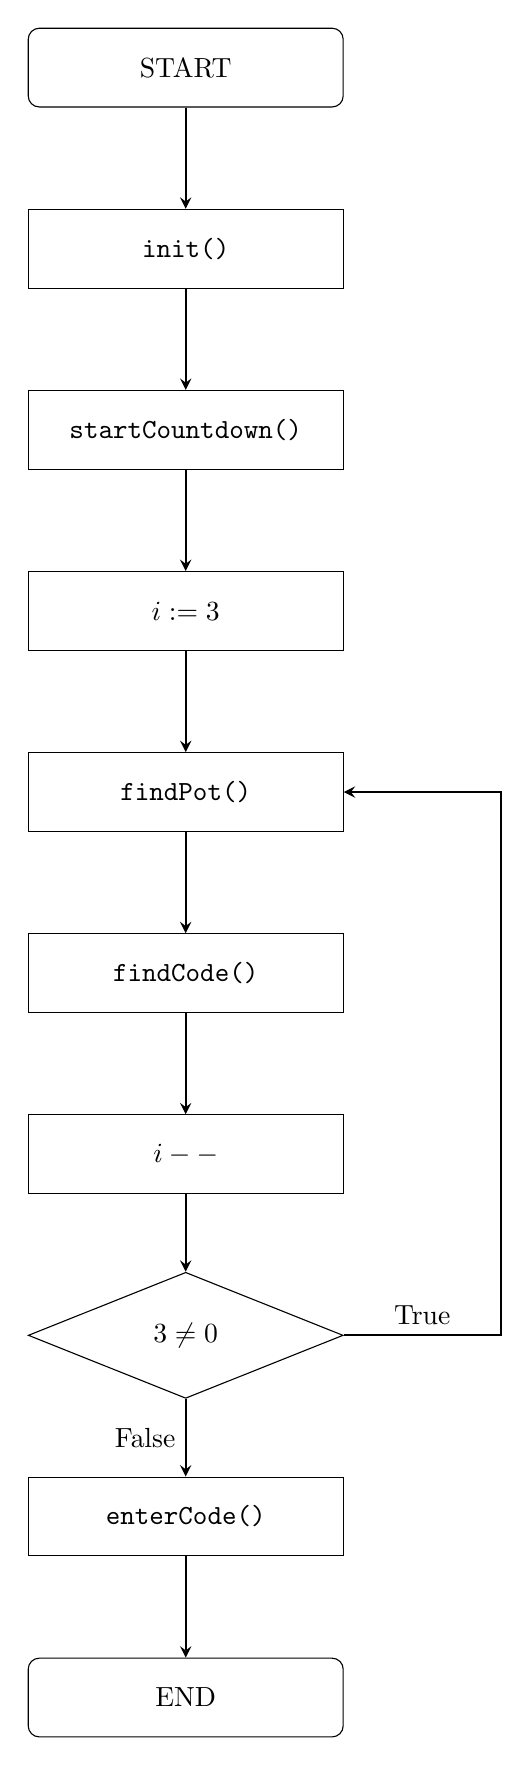
\begin{tikzpicture}[node distance=2.3cm]

	\node (start) [startstop] {START};
	\node (init) [process, below of=start] {\verb|init()|};
	\node (stcd) [process, below of=init] {\verb|startCountdown()|};
	\node (seti) [process, below of=stcd] {$i := 3$};
	\node (pot) [process, below of=seti] {\verb|findPot()|};
	\node (find) [process, below of=pot] {\verb|findCode()|};
	\node (dec) [process, below of=find] {$i--$};
	\node (loop) [decision, below of=dec] {$3 \neq 0$};
	\node (enter) [process, below of=loop] {\verb|enterCode()|};
	\node (end) [startstop, below of=enter] {END};

	\draw [arrow] (start) -- (init);
	\draw [arrow] (init) -- (stcd);
	\draw [arrow] (stcd) -- (seti);
	\draw [arrow] (seti) -- (pot);
	\draw [arrow] (pot) -- (find);
	\draw [arrow] (find) -- (dec);
	\draw [arrow] (dec) -- (loop);
	\draw [arrow] (loop) -- node[anchor=east] {False} (enter);
	\draw [arrow] (loop) -- node[anchor=south] {True} +(4, 0) |- (pot);
	\draw [arrow] (enter) -- (end);

\end{tikzpicture}
\end{center}

\section{Data Structures}

\begin{table}[H]
\centering
\caption{Data Structures Dictionary}
\label{tbl:dict}
\begin{tabular}{@{}lllp{9cm}@{}}
\toprule
Variable Name & Data Type        & Bytes & Description \\ \midrule
\multicolumn{4}{l}{Global Variables} \\ \midrule
fours         & unsigned integer & 1     & Count used by Timer 4 to calculate a second (each count represents 1/30th of a second) \\
bounce        & unsigned integer & 1     & Counter used for debouncing PB1 \\
seed          & unsigned integer & 2     & Seed used for random number generation \\
roundsleft    & unsigned integer & 1     & How many rounds are left in the game \\
at            & enumeration      & 1     & Which round the player is in \\
ocount        & unsigned integer & 1     & Stores the number of seconds per potentiometer round \\ \midrule
\multicolumn{4}{l}{Potentiometer Variables} \\ \midrule
wadc          & flag             & 1     & Stores whether or not the system is waiting on an ADC reading \\
count         & unsigned integer & 1     & Stores the number of seconds left in the last pot round \\
adcreading	& unsigned integer	& 2 & Stores the most recent ADC reading \\  
potwin		& unsigned integer	& 2	& Counter to count 1 second to win the potentiometer round \\ 
temp4:temp3	& unsigned integer	& 2	& Target potentiometer value for the current round \\

\bottomrule
\end{tabular}
\end{table}

\section{Algorithm Descriptions}

The main algorithms used in the program are as follows (shown in C code).

\begin{lstlisting}[language=C, caption={Algorithm for \texttt{startCountdown()}}]

int cdTimer;

void startCountdown() {

	cdTimer = '4';
	do {
		cdTimer--;
		display(cdTimer);
		
		buzzerOn();
		waitms(245);
		buzzerOff();
		waitms(750);
	} while(cdTimer >= '2');
	return;
}		

\end{lstlisting}

\begin{lstlisting}[language=C, caption={Algorithm for \texttt{findPot()}}]

#define IN_POT 2

int seed;
int second;
int count;
int at;
int adcreading;
int potwin;
int wadc;

void timerInterrupt { // timer with a frequency of 32Hz
	if(at == IN_POT){
		if(potwin){
			//increment win countdown
			potwin++;
		}
		if(second == 30) {
			//decrement coundown, check lose condition
			second = 0;
			count--;
			if(!count) {
				lose();
			}
			display(count);

			//turn on the buzzer
			buzzeron();
		} else if(((count == ocount) && (second == 30 >> 1)) || ((count != ocount) && (second == 30 >> 2))) {

			//turn off the buzzer
			buzzeroff();				
		} else if(second & 0b11 == 0 && !wadc) {

			//read from adc
			wadc = 1;
			startReadFromAdc();
		}
	}
	second++;
	return;
}

void resetPot() {
	while(adcreading);
	return;
}

void findPot() {

	at = IN_POT;
	int target = seed; // random number
	target &= 0x3FF;
	reset:
	resetPot();
	while(1) {
		if(adcreading > target) {
			goto reset;
		}
		if(target - adcreading < 48){
			PORTC = 0xff;
		} else {
			PORTC = 0;
		}
		if(target - adcreading < 32){
			PORTG = 0b1;
		} else {
			PORTG = 0;
		}
		if(target - adcreading < 16){

			PORTG = 0b11;
			if(!adcreading) adcreading++;
			if(potwin >= 31) break;
		} else {

			PORTG &= ~0b10;
			potwin = 0;
		}
	}
}

\end{lstlisting}

\section{Module Specification}



\end{document}
